% Chapter 2
\chapter{Bitcoin Transaction Dynamics } % Main chapter title

\label{Chapter2} % For referencing the chapter elsewhere, use \ref{Chapter2} 

\lhead{Chapter 2. \emph{Bitcoin Transaction Dynamics}} % This is for the header on each page - perhaps a shortened title

%----------------------------------------------------------------------------------------
\section{Introduction}

Bitcoin is a decentralized peer to peer electronic payment system in which transactions are performed with no central authority or banks to authorize it. The Bitcoin transactions management and its issuance is carried out collectively by the network. The first Bitcoin specification and proof of concept was published by Satoshi Nakamoto \citep{Nakamoto2008} in 2009 cryptographic mailing list. Bitcoin can also be seen as the most prominent triple entry bookkeeping system in existence. Since then, the community has grown exponentially with many developers working on Bitcoin.


\section{Bitcoin}
\label{sec:bitcoin}
Bitcoin payments use public keys encryption, where, payers and payees are identified by hashed public keys of their Bitcoin wallets. The public keys are generated by ECDSA (Elliptic Curve Digital Signature Algorithm), based on calculations of elliptical curves over finite space. Suppose, Alice sends "$x$" coins to Bob, then an unencrypted transaction attaching Bob's public key is broadcast over the Bitcoin network using her private key. The signature on transaction verifies all users for its authenticity (current owner of coin) by looking at complete history of transactions, called {\it blockchain}. It is essential element in bitcoin architecture, which verifies the legitimacy of ability (sufficient bitcoins) of Alice paying Bob.

\subsection{Blockchain}


The complete record of transactions is in a coded form in a data structure called {\it blockchain}, which is a sequence of records called {\it blocks}. Each block contains a group of transactions that have been sent since the previous block, with integrity check all the way back to the first one, the genesis block.

Any users enter the Bitcoin system by trading non-digital currencies at Bitcoin market exchange, or by mining coins, which involves solving a cryptographically hard problem for which he/she is suitably rewarded a fixed number of Bitcoins  and transactions is validated on the network. The working of mining, core to {\it blockchain}, is mathematically explained better by Johannes et al. \cite{Johannes2015}. The network of peers, called miners, are the agents using computers, who actually add the blocks to the blockchain. Taking example of Alice sending "$x$" coins to Bob from section \ref{sec:bitcoin} by broadcasting over network. The miners receives copies of all transactions as they are generated, including Alice's copy. The blockchain is examined to investigate the history of the bitcoins involved in each transaction. If the proposed transaction from the Alice has sufficient bitcoin credit, then it is accepted for incorporation into the block that the miner is currently working on. 


Identifying each transaction with a double SHA-256 hash, the transactions is gathered together. Then by using miners hashes,together with the hash that is at the current head of the blockchain, as inputs to the cryptographic problem is solved by miners, with rewards of 25 bitcoins in 10 minutes \cite{Johannes2015}. At first, miner~$M$ computes a block hash~$h$ over a unique ordering of the hashes of all the transactions that it is intending to incorporate into its next block $B$.  Then, input of the block solution $s_{i-1}$ is taken at the head of its current version of the {\it blockchain}. If we concatenate the strings by the symbol $+$, the cryptographic problem that $M$ has to solve is: compute a SHA-256 hash
%
\begin{equation} \label{eq:2.1}
s_i = (n + h + s_{i-1}),
\end{equation}
%
such that $s_i$ has at least a specified number~$x$ of leading zeros where $x \sim 64$. 

Once mined, the new block is communicated by broadcasting newly-discovered
blocks via a peer-to-peer network to add the new block at blockchain at each peer using blockchain protocol rules. This makes blockchain as a public ledger, recording  every Bitcoin payment ever made. The simplified version of the whole process is represented in below illustration \ref{fig:blockchain}.

\begin{figure}[ht]
\begin{center}
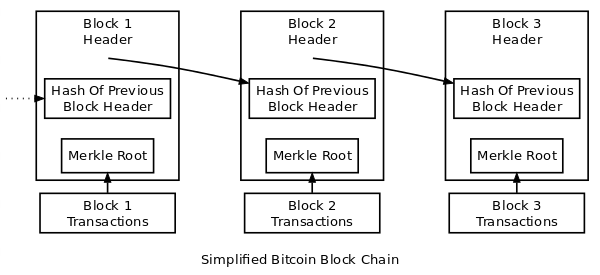
\includegraphics[width=0.8\textwidth]{./Figures/blockchain.png}
\caption{Simple Blockchain \citep{Blockchain2016}}
\label{fig:blockchain}
\end{center}
\end{figure}
The transaction data part of a block consists of one or more new transactions. While the merkel root of the merkle tree contains  hashed copies of each transaction, and the hashes are then paired, hashed, paired again, and hashed again until a single hash remains. The chaining of blocks together and storing the hash of the previous block’s header ensures a transaction cannot be modified without modifying the block that records it and all following blocks. The same goes with the transaction, which are also chained together. A single transaction can create multiple outputs, which  are tied to transaction identifiers (TXIDs), the hashes of signed transactions. Also, the outputs of all transactions included in the block chain can be categorized as either Unspent Transaction Outputs (UTXOs) or spent transaction outputs \ref{fig:block_t}. The first one of these transactions called a generation transaction, which should collect and spend the block reward (comprised of a block subsidy and any transaction fees paid by transactions included in this block). All these transactions are encoded into blocks in binary rawtransaction format, making it difficult for researchers to extract in simple relational database format, to get transaction graph.

\begin{figure}[ht]
\begin{center}
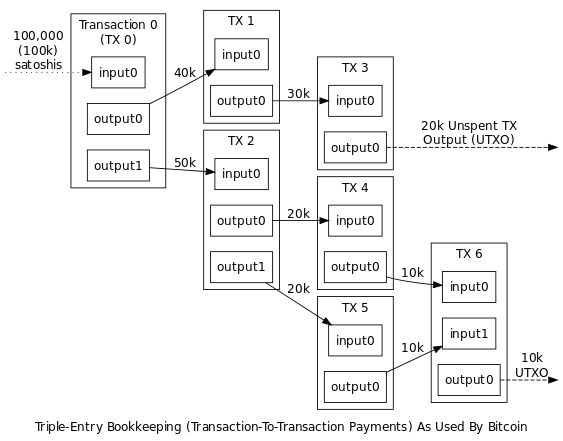
\includegraphics[width=0.8\textwidth]{./Figures/block_t.png}
\caption{Blockchain Transaction \citep{Blockchain2016}}
\label{fig:block_t}
\end{center}
\end{figure}

\section{Related Work}
The possibility to analyze agent resolved transactions in any market is limited by the scarcity of available data, as this kind of information is usually considered highly sensitive. But with the publicly available blockchain at every machine allows researchers to reconstruct the network of transactions and extract the time and amount of each payment. There are many research studies that concerns bitcoin transaction network using network analysis, machine learning and statistical physics techniques.

Parsing four (2009-2013) years data from bitcoin's  blockchain, Kondor et al. \citep{Csabai2014}  analyze the structure of the transaction network by measuring network characteristics over time, such as the degree distribution, degree correlations, clustering and money movement. Using the same data, they in their different paper \citep{Kondor2014} analyze changes in the structure of the subgraph induced by the most active users. They were  able to show find correlation between structural changes in the network and exchange price of bitcoins. But with exponential increase in the number of transaction over years, they method seems obsolete , as it is difficult to scale with their endorsed methods.

Reid and Harrigan \citep{Reid2013} linked addresses belonging to the same entity using external information. The using techniques such as context discovery and flow analysis, they investigate an alleged theft of Bitcoins. By running the Union-Find algorithm, Ron and Samir \citep{Ron2013}  associated the 3,120,948 addresses with 1,851,544 different entities to understand behaviour of users. Spagnuolo \citep{Spagnuolo2013} released open source project Bitiodine, which was able to cluster addresses and classify them using a dataset partially obtained in an automatic fashion, using scrapers for major web sources of bitcoin addresses. On the similar line, other paper \citep{Fleder2015} investigates bitcoin transaction-graph-annotation, which is capable of tracing and clustering user activity.

Most of the  previous research employed data collected from old Bitcoin- client Bitcoin 0.8 later, the newer bitcoin clients indexed the full blockchain using LevelDB instead making the publicly available bitcointools obsolete. Adding to the same, the nearing 300,000 transactions/day in 2015 gives really hard time to earlier algorithms to scale, thus motivating us to develop new techniques to parsing data from blockchain, reconstructing network and doing analysis.

\section{Data}
\label{data}
The blockchain is a transaction database of the Bitcoin.  Once Bitcoin core is setup at local machine, blockchain is automatically downloaded. Every full node participating in the Bitcoin network has the same copy. As of now there is more than 60 GB of Bitcoin blockchain dataset, which makes it difficult to parse the raw blockchain data. Most of the previous studies \citep{Ron2013} employed a forked version of bitcointools \footnote{\url{https://github.com/gavinandresen/bitcointools}}, but from the bitcoin clients 0.8 version, it indexed the full blockchain using LevelDB instead making the publicly available bitcointools obsolete. Other well know open source blockchain parser like blockparser \footnote{\url {https://github.com/znort987/blockparser}}, BitIodine \citep{Spagnuolo2013} etc are almost undocumented projects, where some appear to not even work. A paper \citep{Fleder2015} led me to BitcoinArmory project, which requires a dozen of manual interventions to get installed, but still doesn’t work.

We then started to look for ready-made SQL database, which pointed to BitcoinABe. This python based library reads the Bitcoin block file, transforms and loads the data into a SQL database \ref{fig:SQL}. But, Its takes more than two weeks to dump the data, which was not feasible option. We downloaded postgres database dumps of the bitcoin-ruby-blockchain database generated by webbtc \footnote{\url{http://dumps.webbtc.com/bitcoin/}}. Then, with slight modification to open repository BitIodine \citep{Spagnuolo2013} code, we parsed through the blockchain, and wrote wrapper classes that extracted the relevant information required to construct the transaction graph. The market price data was scarped from website \url {https://blockchain.info/} to plot graphs in R.

\section{Bitcoin Transaction Network}

Before getting the transaction network, we first define our graph, which acts as input to further mathematical application.

\begin{definition}
We consider weighted labelled graph. That is, a
graph $G=(V,E,\ell)$ is represented by a set of $|V|=n$ vertices, a
set of edges $E$ specified by a weighted adjacency matrix $A \in
\bb{R}^{n \times n}$, and a label function $\ell\colon V \rightarrow
\cm{L}$ with $\cm{L} = \left( [k], \R^D \right)$, where $k$ is the
number of available node labels and $D$ is the dimension of the
continuous attributes.  Given $V = \{v_1,v_2,...,v_n\}$, \emph{node
  labels} $\ell(v_i)$ are represented by nominal values and
\emph{attributes} $\mathbf{x}_i \in \bb R^D$ are represented by
continuous vectors. In a transaction graph, addresses are nodes, transactions are edges and weight is BTC.
\label{def:graph}
\end{definition}

With the overall transactions records parsed from the blockchain in human readable form, we construct a a weighted directed transaction graph that gives an intuition towards the flow of Bitcoins from one key to the other,the directed edge represents a particular transaction from a source address to a target address and weight represents the value of the transactions. For our experiments, we constructed graphs for more than two years (March, 2013 to December, 2015) to capture major bubble in Bitcoin history. Figure \ref{fig:dt} represent daily transaction graph for a typical day on April 8, 2013.

\begin{figure}[ht]
\begin{center}
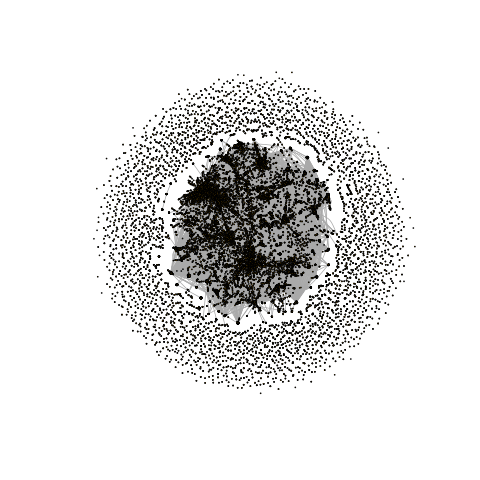
\includegraphics[width=\textwidth]{./Figures/dt.png}
\caption{ Daily transaction graph for a typical day (April 8, 2013)}
\label{fig:dt}
\end{center}
\end{figure}

\section{Transaction Dynamics}
The validation of the data parsed from our tool is then checked by
reproducing the ”Mathew Effect” phenomenon from the seminal work of Kondor et al. \citep{Csabai2014} paper’s using their original matlab code, but with our own data. The authors of the above papers are curator of whole blockchain up to 2014.10.19. (326,027 blocks), which is benchmark in quality. The similar figure confirms the high quality of our data.

To capture the transaction  dynamics in the bitcoin, we analyze the dynamics of money flow on the transaction network, as discussed in the paper \citep{Csabai2014}. We try to support popular hypothesis in economics having roots in preferential attachment, called Matthew effect or the "rich get richer phenomenon". It states that the growth of the wealth of each individual is proportional to the wealth of that individual \citep{Csabai2014}.

We assume that the number of bitcoins associated with node $n$ at time $t$ is given by $b_{n}(t)$. The difference between the balance of each
address at the end and at the start of each month is calculated. Then the difference in function of the starting balances is plotted in figure \ref{fig:dynamics}. The  positive correlation between balance and the average growth indicates the "rich get richer" phenomenon in bitcoin.

\begin{figure}[ht]
\begin{center}
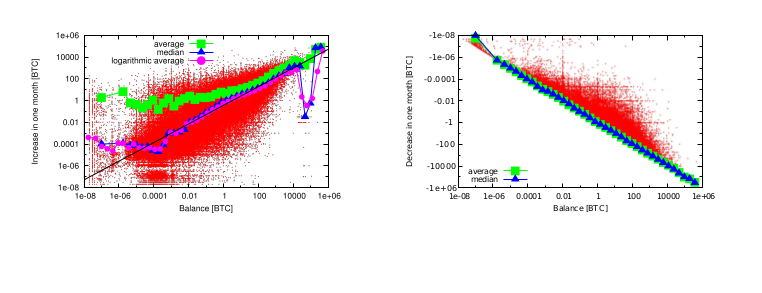
\includegraphics[width= \textwidth]{./Figures/dynamics.png}
\caption{ Matthew Effect}
\label{fig:dynamics}
\end{center}
\end{figure}

The figure \ref{fig:dynamics} is reproduced from Kondor's paper \citep{Csabai2014}, using our own data where Increase (left) and decrease (right) of node balances in one month windows as a function of their balance at the beginning of each month is represented. The representation in the picture follow the following colors: the raw data (red), the average (green), median (blue) and logarithmic average (magenta). The later three are calculated for logarithmically sized bins. The power-law fit for the double logarithmic data is represented by black line.

\subsection{Silk Road Arrest}

The Silk Road, under the alias of “Dread Pirate Roberts” (DPR) was known as an anonymous marketplace, a Black Market operated as a hidden service only accessible through Tor, where people who use bitcoins were able to buy and sell drugs, art, weapons etc. anonymously, without the risk of being tracked. It was founded by Ross William Ulbricht in February in 2011, but in October 2013 FBI closed the Silk Road and arrested Ulbricht. The FBI  seized approximately 173,600 BTC in two phase. At the first go 29,600 BTC held in a so called hot wallet were seized and an additional 144,000 BTC were seized using two addresses \footnote{1F1tAaz5x1HUXrCNLbtMDqcw6o5GNn4xqX, 1FfmbHfnpaZjKFvyi1okTjJJusN455paPH} controlled by the FBI. 

We illustrates the event using transaction network \ref{fig:silk} realised in gephi. Each vertex represents a user, where address is mapped to the user. Each directed edge between a source and a target represents a flow of Bitcoins from a public-key belonging to the user corresponding to the source to a public-key belonging to the user corresponding to the target. 

\begin{figure}[ht]
\begin{center}
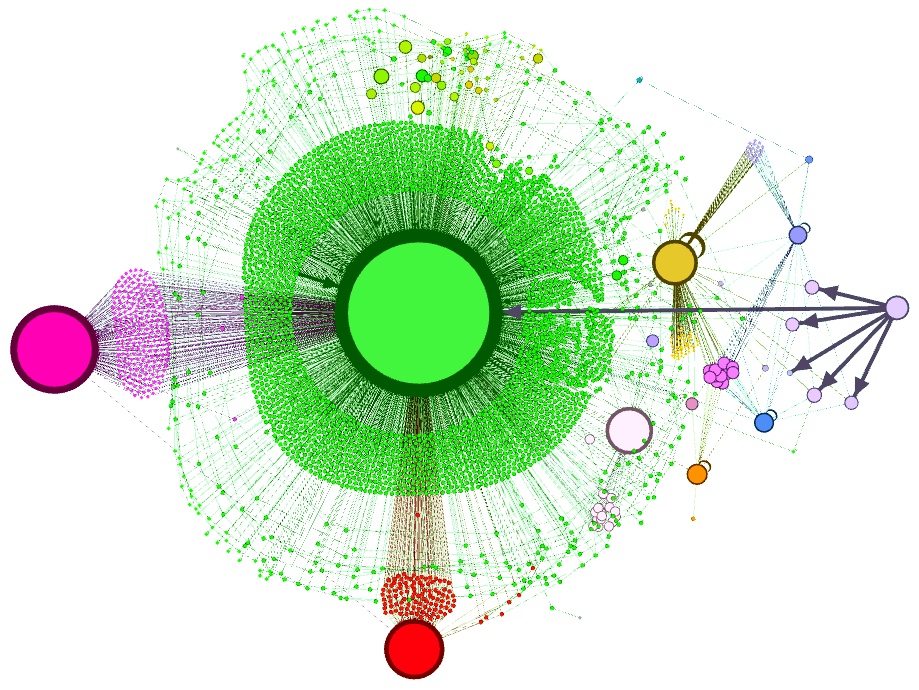
\includegraphics[width=0.7\textwidth]{./Figures/silk.png}
\caption{ Silk Road Arrest}
\label{fig:silk}
\end{center}
\end{figure}

Although in this scenario involves manual investigation by web scraping , it would have been difficult to find significant links manually, given the millions of nodes involved.

\section{Summary}
This chapter introduces Bitcoin, its working detail by explaining the protocol of blockchain, which contains all the history of transactions in the bitcoin. With enough knowledge about working of bitcoin, the related work in bitcoin transaction network is the discussed with the pros and cons. The data preparation staged is discussed to get the transaction network, an input to our mathematical model in coming chapters. The case study of silk road arrest is illustrated with the transaction graph. Transaction dynamics is reproduced from know studies to validate the parsed data, concludes the chapter.